\newpage

\begin{center}
	\section{Resultado}
\end{center}

\noindent
\justify

Conociendo la distribuci\'on geom\'etrica de las aletas que mejor distribuci\'on de energ\'ia y mayor magnitud de energ\'ia de impacto por tipo de bola produce, se desarroll\'o una nueva simulaci\'on num\'erica con el material a pulverizar (agente dispersante y material vegetal) para detallar la forma en c\'omo se distribuye el material durante la etapa de molienda. La proporci\'on de llenado, en t\'erminos volum\'etricos, es la siguiente: $20\%$ lo ocupan las bolas del molino, $16\%$ el material vegetal y el $14\%$ el agente dispersante.

\begin{figure}[h!]
	\centering
	\begin{subfigure}[b]{0.6\textwidth}
		\centering
		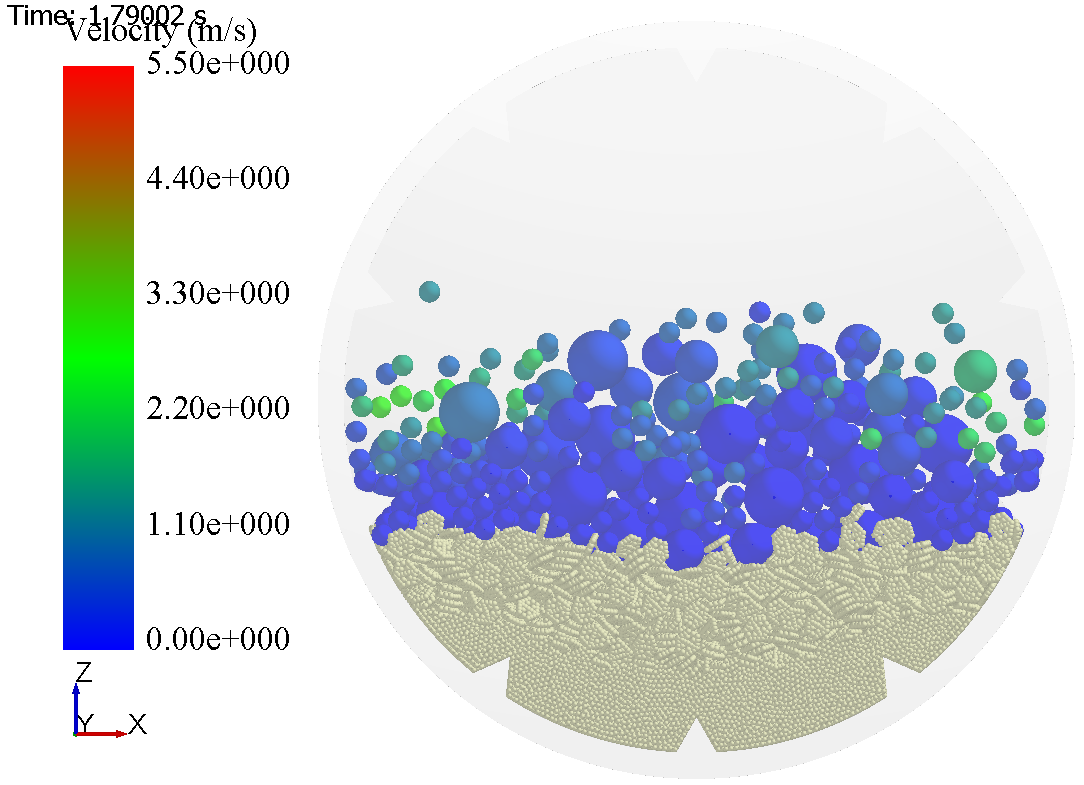
\includegraphics[width=\textwidth]{Images/Resultados/Real.PNG}
		\caption{Material a moler.}
	\end{subfigure}
	\hfill
	\begin{subfigure}[b]{0.6\textwidth}
		\centering
		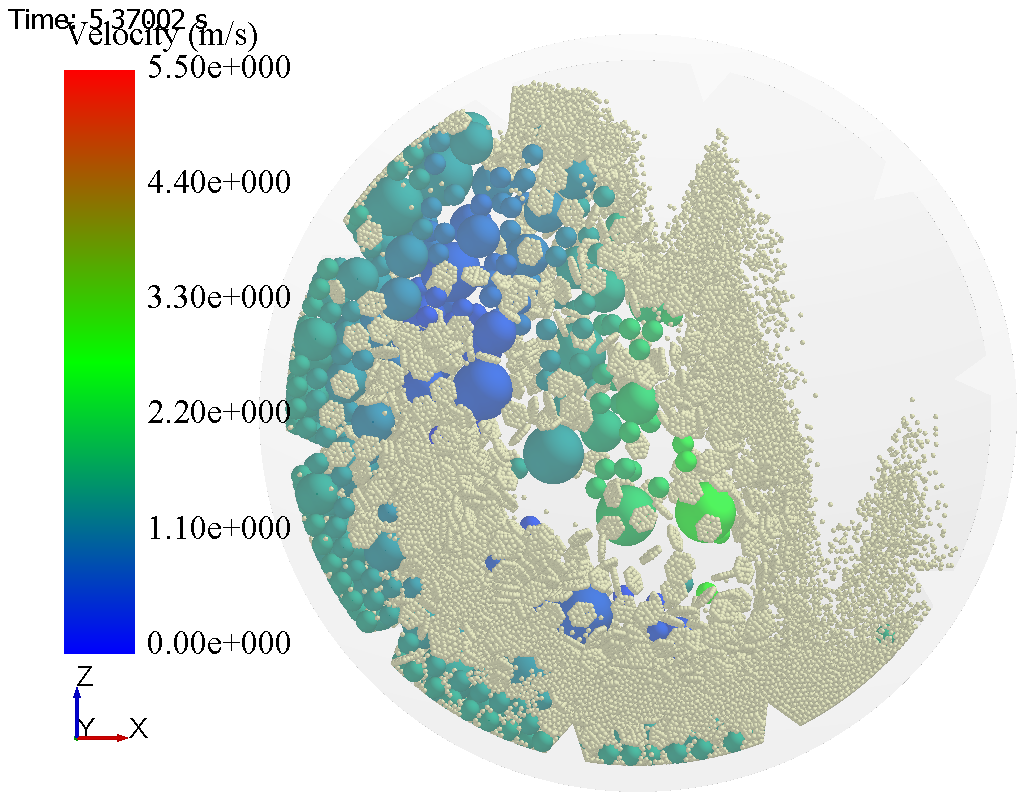
\includegraphics[width=\textwidth]{Images/Resultados/total.PNG}
	\caption{Molienda.}
	\end{subfigure}
	\caption{Simulaci\'on con el material a pulverizar.}
	\label{resul4}
\end{figure}


